\documentclass[paper=a4, fontsize=12pt, svgnames]{scrartcl}

\usepackage[utf8]{inputenc}
\usepackage{amsmath,amsfonts,amsthm,bm} % Math packages
% to include graphics & make the path to images shorter
\usepackage[pdftex]{graphicx}
\graphicspath{{images/}}
% to write code with appropriate fonts
\usepackage{listings}
\usepackage{color}
% to make colores in title page
\usepackage{tikz}
\usetikzlibrary{trees}

\allsectionsfont{\centering \normalfont\scshape}



\newcommand{\be}[1]{\begin{equation}\label{#1}}
\newcommand{\ee}{\end{equation}}
\newcommand{\ba}[1]{\begin{eqnarray}\label{#1}}
\newcommand{\ea}{\end{eqnarray}}
\newcommand{\rf}[1]{(\ref{#1})}
\newcommand{\angstrom}{\textup{\AA}}



\title{Report for FYS-STK4155: Project 1}
\author{maxim.brilenkov }
\date{October 2019}

\begin{document}


\lstset{language=Python,
 basicstyle=\ttfamily,
 keywordstyle=\color{red},
 %commentstyle=\color{darkgreen},
 morecomment=[l]{!},
 showstringspaces=true,
 frame=single,
 basicstyle=\ttfamily\footnotesize,
 breaklines=true,
 postbreak=\raisebox{0ex}[0ex][0ex]{\ensuremath{\color{red}\hookrightarrow\space}},
 %directivestyle=\color{magenta}\ttfamily,
 emph={int,char,double,float,unsigned},
 emphstyle=\color{blue},
 firstnumber=1, % Line numbers start with line 1
 stepnumber=5 % Line numbers go in steps of 5
} 



\maketitle

\begin{abstract}
    \textit{Abstract: accurate and informative? }
    The abstract gives the reader a quick overview of what has been done and the most important results. Try to be to the point and state your main findings.
    
    In this work, I have written the code, which implements several regression algorithms, namely \textit{Linear Regression}, \textit{Ridge Regression} and \textit{LASSO regression}. Th code has been tested firstly on the artificial and then on the real data - Norwegian terrain.
\end{abstract}

%%%%%%%%%%%%%%%%%%%%%%%%%%%%%%%%%%%%%%%%%%%%%%%%%%%%%%%%%
\section{Introduction}
\label{introduction}

%\textit{Introduction: status of problem and the major objectives.}

%When you write the introduction you could focus on the following aspects

%Motivate the reader, the first part of the introduction gives always a motivation and tries to give the overarching ideas
%What I have done
%The structure of the report, how it is organized etc



\textbf{Machine Learning} (ML) is a rapidly developing field of Science, which, in some cases (e.g. \textit{Optical character recognition}), has been around for decades already. However, it is impact on a various fields, such as: Technology, Humanities, Medicine, Law, Social sciences etc. cannot be overrated. Its applications ranges from development of self-driving cars to solving complicated numerical problems and thus are perceived by many as one of main tools in modern world. 

But what is Machine learning? It can have a variety of definitions. O'Reilly \textit{et al} \cite{Geron} defines it as "\textit{the science (and art) of programming computers so they can learn from data}". Based on the data we have and the outcome we want to have, ML systems can be classified into several broad categories \cite{Geron}: 
\begin{itemize}
    \item \textit{Supervised}, \textit{unsupervised} or \textit{semi-supervised} ML algorithms. This approach describes whether or not the pipeline is trained with human interference/supervision; 
    \item \textit{Online}/\textit{batch} learning. This approach describes whether or not they can learn incrementally on the fly;
    \item \textit{Instance-based}/\textit{Model-based} learning. This approach describes whether they work by simply comparing new data points to known data points, or instead detect patterns in the training data and build a predictive model.
\end{itemize}

This entire project was based on the \textit{supervised} learning algorithms, where you have an input variable(s) (also known as \textit{features}/\textit{predictors}), $\bm{x}=[x_0, x_1, x_2,...x_{n-1}]^T$, and an output variable(s) (\textit{response}/\textit{outcome}), $\bm{y}=[y_0, y_1, y_2,...,y_{n-1}]^T$, and you use an algorithm to learn the mapping function from the input to the output $Y = f(X)$. Such a task is called \textit{regression} and in this report I have studied three different \textit{Linear Regression} algorithms - Polynomial, Ridge and LASSO regression.

I have written the code, which implements all of the three above mentioned fitting procedures. First, I manually generate the data set on a grid and then tried to fit the system's response, which is represented in terms of Franke function \cite{Morten}. Later, I calculate the regression coefficients and their respective confidence intervals, together with associated its respective errors. Afterwards I talk about k-Fold cross validation as well as \textit{bias-variance trade-off}. In addition, I talk about their advantages and disadvantages, while comparing my results with Scikit Learn functionality.

The report organized as follows. In section \ref{sec:formalism}, I briefly state the formalism of the problem. Section \ref{sec:code_imp} explains the idea behind the code. In section \ref{sec:results}, I analyze results I have obtained. The conclusion and discussion are given in \ref{sec:conclusions}. The code is listed in the end of this report.

\section{Formalism}
\label{sec:formalism}

%\textit{Formalism/methods: Discussion of the methods used and their basis/suitability.}

In this section, I briefly remind the reader about the theoretical background of the problem. For more thorough discussion please refer to \cite{Morten} and/or \cite{Hastie} (lecture notes and elements of statistical learning).

%Regression: Finding a functional relationship between an input data set and a reference data set. The goal is to construct a function that maps input data to continuous output values. (Ref. Lecture notes)

\subsection{Polynomial Regression}

To do the regression analysis means to find a functional relationship between data set and a reference set \cite{Morten}. Therefore, the aim of the regression analysis is to \textit{construct the function}, which will, in principle, map any input data of a similar format to some continuous output values. To put it simply, we want to describe given data set in terms of some variables and not only that, but also to have a model which will be able to predict similar values. Thus, we need to construct the function in such a way, which will allow us to predict the values $y$ not present in the current set. The most basic idea then is to parametrise the function in terms of polynomial. If we have $n$ points, we get $n-1$ (first is zero degree, i.e. constant), which results in \cite{Morten}:
\be{1}
y(x_i) = \tilde{y}_i + \epsilon_i=\sum_{j=0}^{n-1}\beta_jx_i^j+\epsilon_i\, ,
\ee
Using matrix notation, this expression can be written as \cite{Morten} :
\be{2}
\bm{y} = \bm{X\beta} + \bm{\epsilon}\, ,
\ee
where
\be{3}
\bm{y} = [y_0,y_1,...,y_{n-1}]^T, \quad \bm{\beta} = [\beta_0,\beta_1,...,\beta_{n-1}]^T, \quad \bm{\epsilon} = [\epsilon_0,\epsilon_1,...,\epsilon_{n-1}]^T\, ,
\ee
\[
\bm{X} =
  \begin{bmatrix}
    x_{00} & x_{01} & x_{02} & ... & x_{0,n-1} \\
    x_{10} & x_{11} & x_{12} & ... & x_{1,n-1} \\
    ... & ... & ... & ... & ... \\
    x_{n-1,0} & x_{n-1,1} & x_{n-1,2} & ... & x_{n-1,n-1} \\
  \end{bmatrix}
\]
The idea is to obtain an optimal set of $\beta_i$ values, which can fit best our current and future datasets. We do this by defining an approximation
\be{4}
\bm{\tilde{y}}=\bm{X\beta}\, ,
\ee
and minimising the so-called \textit{cost function}
\be{5}
\bm{C}(\bm{\beta}) = \frac{1}{n}\sum_{i=0}^{n-1}\left(y_i-\tilde{y}_i\right)=\frac{1}{n}\bm{\left\{\left(y-\tilde{y}\right)^T\left(y-\tilde{y}\right)\right\}}\, ,
\ee
i.e. by minimizing the square distance between the estimated function and the observed value, also known as \textit{residual sums of squares}
\be{}
\hat{\bm{\beta}}=\text{arg min}_\beta \bm{\left\{\left(y-\bm{X\beta}\right)^T\left(y-\bm{X\beta}\right)\right\}}\, ,
\ee
Such optimization problem has the solution in the form \cite{Morten}
\be{6}
\bm{\hat{\beta}} = \left(\bm{X^TX}\right)^{-1}\bm{X^Ty}\, .
\ee
$\bm{\hat{\beta}}$ is known as \textit{ordinary least squares estimator}, and due to the common assumption that the error term, $\varepsilon$, has mean zero, the OLS estimator supposed to be \textit{unbiased}. Such property allows OLS to evaluate the \textit{true} values of the regression coefficients.

Sometimes matrix $\bm{X^TX}$ cannot be inverted and thus the standard OLS, based on inversion algorithm, will lead to singularities. One of approaches to avoid this is called \textbf{Singular Value Decomposition}, which allows us to rewrite $X$ in terms of an orthogonal/unitary transformation $U$ \cite{Morten}
\be{7}
\bm{X}=\bm{U\Sigma V^T}\, ,
\ee
With this in mind, it can be shown that \cite{Morten} 
\be{8}
\bm{X\beta}=\bm{X}\left(\bm{VDV^T}\right)^{-1}\bm{X^Ty}=\bm{U\Sigma V^T}\left(\bm{VDV^T}\right)^{-1}\left(\bm{U\Sigma V^T}\right)^T\bm{y}=\bm{UU^Ty}\, .
\ee

\subsection{The Bias-variance trade-off}

In principle, we want to estimate the regression coefficients with the method, which involves least possible errors. The prediction error is frequently introduced by the metric called \textit{Mean Squared Error} (MSE) and it can be defined as \cite{Morten}

\be{16}
\text{MSE}(\bm{X\beta})=E\left[\left(\bm{y}-\tilde{\bm{y}}\right)^2\right], \quad \bm{y} = \bm{f}(\bm{x}) + \bm{\varepsilon}\, ,
\ee
Let us look into this expression in a more detail
\ba{17}
E\left[\left(\bm{y}-\tilde{\bm{y}}\right)^2\right]&=&E\left[\left(\bm{f}+\bm{\varepsilon} - \tilde{\bm{y}}+E[\tilde{\bm{y}}] - E[\tilde{\bm{y}}]\right)^2\right]\nn\\
&=&\left[\left(\bm{f}-E[\bm[y]]\right)-\left(\tilde{\bm{y}}-E[\tilde{y}]\right)\right]^2 + \sigma^2\nn\\
&=&\left(\bm{f}-E[\bm{y}]\right)^2-2\left(\bm{f}-E[\bm{y}]\right)\left(\tilde{\bm{y}}-E[\tidle{\bm{y}}]\right)+\left(\tilde{\bm{y}}-E[\tilde{\bm{y}}]\right)^2+\varepsilon^2\nn\\
&=&E\left[\left(\bm{f}-E[\bm{y}]\right)^2+\left(\tilde{\bm{y}}-E[\tilde{\bm{y}}]\right)^2+\bm{\varepsilon}^2\right]-2E\left[\left(\bm{f}-E[\bm{y}]\right)\left(\tilde{\bm{y}}-E[\tidle{\bm{y}}]\right)\right]\, ,
\ea
where the last part equals to zero because:
\be{18}
E[\bm{f}E[\tilde{\bm{y}}]]=E[\bm{f}]E[\bm{\tilde{y}}]\, ,
\ee
Thus, we get
\be{19}
\text{MSE}(\bm{X\beta})=E\left[\left(\bm{y}-\tilde{\bm{y}}\right)^2\right]=E\left[\left(\bm{f}-E[\bm{y}]\right)^2+\left(\tilde{\bm{y}}-E[\tilde{\bm{y}}]\right)^2+\bm{\varepsilon}^2\right]\, ,
\ee
or
\be{20}
E\left[\left(\bm{y}-\tilde{\bm{y}}\right)^2\right]=\frac{1}{n}\sum_i\left(f_i-E[\tilde{\bm{y}}]\right)^2+\frac{1}{n}\sum_i\left(\tilde{y}_i-E[\tilde{\bm{y}}]\right)^2+\sigma^2\, .
\ee
The last term, $\sigma^2$ here irreducible error and it is beyond our control. The second term is the \textit{variance} of our model, which is simply the variance of the an average. It decreases with inverse of n (the degrees of freedom/model complexity). The first term is \textit{bias} and it is the squared difference between the true mean and the expected value of the estimate. As $n$ grows, it will increase; hence the \textir{bias-variance trade-off}.

Because of the existence of bias-variance trade-off, it could be better if we would be able to utilize this property somehow. We can do this by introducing bias to the estimates, while achieving less variability. Unfortunately, OLS are unbiased by default and hence cannot be exploited. 

But what if we introduce this bias? For instance, adding the penalty, $\lambda$:
\be{9}
\bm{X^TX}\rightarrow\bm{X^TX}+\bm{\lambda I}\, ,
\ee
It can be shown (see e.g. \cite{Hastie}, that in this way we will get a slightly different optimization problem:
\be{}
\hat{\bm{\beta}}^{\text{ridge}}=\text{arg min}_\beta \left\{\bm{\left(y-\bm{X\beta}\right)^T\left(y-\bm{X\beta}\right)} + \lambda\sum_{i=1}^p\beta_i^2\right\}}\, ,
\ee
or
\be{11}
\hat{\bm{\beta}}^{\text{ridge}}=\left(\bm{X^TX} + \lambda\bm{I}\right)^{-1}\bm{X}^T\bm{y}\, ,
\ee
Such optimization problem is called \textbf{Ridge} regression and it is highly dependable on the \textit{tuning} or \textit{penalty} (\textit{hyper}) parameter, $\lambda$.

Ridge regression is the part of \textit{shrinkage methods} \cite{Hastie} and it imposes the penalty on the size of regression coefficients and thus shrinks them. The amount of shrinkage is controlled by $\lambda \ge 0$ - larger $\lambda$ leads to larger amount of shrinkage.

In addition, $\lambda$ is not affected by the learning algorithm itself and must be set before start training the algorithm. Moreover, its value should remain constant during the entire training process.

Very large values of $\lambda$ will result in almost flat model (zero slope); thus, it will not achieve \textit{overfitting} of the training data, but there is smaller chance to find a good solution.

\subsection{LASSO regression}

The LASSO (Least Absolute Shrinkage and Selection Operator) is a regression method that involves penalizing the absolute size of the regression coefficients.

By penalizing or constraining the sum of the absolute values of the estimates you make some of your coefficients zero. The larger the penalty applied, the further estimates are shrunk towards zero. This is convenient when we want some automatic feature/variable selection, or when dealing with highly correlated predictors, where standard regression will usually have regression coefficients that are too large.

Lasso is quite different in comparison to Ridge, i.e. the estimate now defined as \cite{Hastie}:
\be{14}
\hat{\beta}^{lasso} = \text{argmin}_\beta\sum_{i=1}^N\left(y_i-\beta_0-\sum_{j=1}^px_{ij}\beta_j\right)^2\, ,
\ee
\be{15}
\text{subject to}\sum_{j=1}^p|\beta_j|\le t\, ,
\ee
In this case the solution for $\hat{\beta}^0=<y>$ which means we need to fit our model without an intercept, and thereafter we fit a model without an intercept.

To summarize, while Ridge regression does a proportional shrinkage, Lasso translates each coefficient by a constant factor $\lambda$ truncating at zero \cite{Hastie}.

%For Lasso you can simply state that it optimizes the learning rate, that is it finds the optimal learning rate via various methods

%https://scikit-learn.org/stable/modules/sgd.html

\subsection{Resampling Methods - Cross validation}

Splitting your data set into test and training one is the common practice in ML algorithms. It is used to compare and select a model for a given predictive modeling problem because it is easy to understand, easy to implement, and results in skill estimates that generally have a lower bias than other methods \cite{Geron} (hands on machine learning).

There are a lot of ways to split your data set into several parts. One of them is called \textbf{k-Fold Cross validation} (CV). It is a statistical method used to estimate the "learning" skill of ML models. It is very useful resampling if you have limited data sample and you want to test your model. It is called k-Fold because the parameter k refers to the number of groups that a given data sample is splitted into. When a specific value for e.g. k=10 is chosen, k-Fold becomes 10-fold CV.

After you splitted your entire data set on k subsets, you train each model against different combination of these subsets and validate it against the remaining parts. Once the model type and $\lambda$ have been selected, a final model is trained using these hyperparameters on the full training set, and the generalized error is measured on the test set. 

It is primarily used  to estimate the skill of ML model on "unseen" data, i.e. you have a limited sample and you use it estimate how well your model will work in general on the data, which were not used during the training of the model.

Overall, the algorithm is fairly straightforward:
\begin{itemize}
    \item Shuffle the data set randomly;
    \item Split the data set into k groups;
    \item For each unique group:
    \begin{enumerate}
        \item Take the group as a hold out or test data set;
        \item Take the remaining groups as a training data set;
        \item Fit a model on the training set and evaluate it on the test set;
        \item Retain the evaluation score and discard the model;
        \item Summarize the skill of the model using the sample of model evaluation scores.
    \end{enumerate}
\end{itemize}





\section{Code implementation and testing}
\label{code_imp}

\textit{Code/Implementations/test: Readability of code, implementation, testing and discussion of benchmarks.}
\begin{itemize}
    \item Describe the methods and algorithms
    \item You need to explain how you implemented the methods and also say something about the structure of your algorithm and present some parts of your code
    \item You should plug in some calculations to demonstrate your code, such as selected runs used to validate and verify your results. The latter is extremely important!! A reader needs to understand that your code reproduces selected benchmarks and reproduces previous results, either numerical and/or well-known closed form expressions.
\end{itemize}

In this section I describe the various parts of the code I've written. It equally works for fake (manually generated) and real (Norwegian terrain) data sets. The whole folder structure can be viewed as follows:
\begin{itemize}
    \item reglib.py - small library, which contains all necessary methods to calculate $\beta$'s, MSE, CrossValidation and Bias-Variance trade-off;
    \item regression.py - main module, which contains the entry point of the program together with calling procedures for the reglib.py library;
\end{itemize}

\tikzstyle{every node}=[draw=black,thick,anchor=west]
\tikzstyle{selected}=[draw=red,fill=red!30]
\tikzstyle{optional}=[dashed,fill=gray!50]
\begin{center}
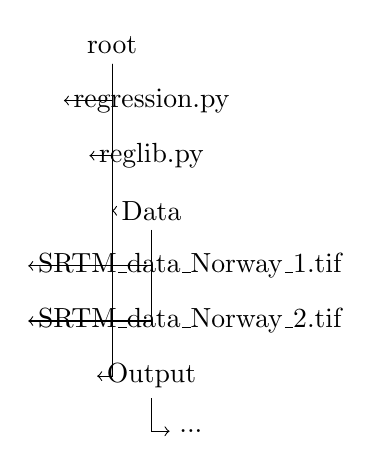
\begin{tikzpicture}[
  grow via three points={one child at (0.5, -0.7) and
  two children at (0.5, -0.7) and (0.5,-1.4)},
  edge from parent path={[->](\tikzparentnode.south) |- (\tikzchildnode.west)}]
    \node {root}
    child { node {regression.py}}		
    child { node {reglib.py}}
    child { node {Data}
        child { node {$\mathrm{SRTM\_data\_Norway\_1.tif}$} }
        child { node {$\mathrm{SRTM\_data\_Norway\_2.tif}$} }
    }
    % adding these to make some space
    child [missing] {}				
    child [missing] {}				
    child { node {Output}
        child { node {...} }
    };
\end{tikzpicture}
\end{center}
\begin{itemize}
    \item \textbf{reglib.py} - small library, which contains all necessary methods to calculate $\beta$'s, MSE, CrossValidation and Bias-Variance trade-off;
    \item \textbf{regression.py}  - main module, which contains the entry point of the program together with calling procedures for the reglib.py library;
    \item \textbf{Data} - folder which contains the real data. Note: you do not necessarily need to copy the data files inside, but can use the full path in your OS;
    \item \textbf{Output} - contains all the output files produced during the program run.
\end{itemize}

To obtain the program please navigate to the directory you want the program to be stored at with:
\begin{lstlisting}
cd /path/to/your/directory/
\end{lstlisting}
and simply clone the repository by typing:
\begin{lstlisting}
git clone https://github.com/maksymbr/machine-learning-projects.git
\end{lstlisting}

The script was written and tested with python 3.7. I was running it either through JupyterNotebook, Spider or PyCharm. But, it is possible to run it through terminal. Just locate to the directory with the script and type:
\begin{lstlisting}
python regression.py
\end{lstlisting}

After execution, you will be asked some questions about the data set and other parameters you want to use. In my opinion, it is quite quite simple to understand, so I will omit the tedious explanations here and will go straight to the code explanation.

\subsection{Fake Data}

The original idea was to write a program which, in principle, will be able to work with any amount of independent variables. For this I am using a sympy library to generate the \textit{symbolic} array of independent variables as:
\begin{lstlisting}
x_symb = sp.symarray('x', n_vars, real = True)
\end{lstlisting}
which will result in a list of variables $x_0$, $x_1$, $x_2$, ... $x_n$, where $n=\mathrm{n\_vars}$.

For a given set of points, I am generating a set of values for the symbolic variables as follows:
\begin{lstlisting}
x_vals = x_symb.copy()
for i in range(n_vars):
    x_vals[i] = np.arange(0, 1, 1./N_points)
\end{lstlisting}
Because we are using Franke function (\ref{} lecture notes):
\begin{lstlisting}
def FrankeFunction(x,y):
    term1 = 0.75*np.exp(-(0.25*(9*x-2)**2) - 0.25*((9*y-2)**2))
    term2 = 0.75*np.exp(-((9*x+1)**2)/49.0 - 0.1*(9*y+1))
    term3 = 0.5*np.exp(-(9*x-7)**2/4.0 - 0.25*((9*y-3)**2))
    term4 = -0.2*np.exp(-(9*x-4)**2 - (9*y-7)**2)
    return term1 + term2 + term3 + term4
\end{lstlisting}
I am generating the response as:
\begin{lstlisting}
import reglib as rl
# library object instantiation
lib = rl.RegressionLibrary(x_symb, x_vals)
# setting up the grid
x, y = np.meshgrid(x_vals[0], x_vals[1])
# and getting output based on the Franke Function
z = lib.FrankeFunction(x, y) + 0.1 * np.random.randn(N_points, N_points)
\end{lstlisting}
and, for each polynomial (up to specified max value), I am instantiating the pipeline, which calculates OLS, Ridge and LASSO regressions with several different hyper parameters
\begin{lstlisting}
for poly_degree in range(1, max_poly_degree+1):
    print('\n')
    print('Starting analysis for polynomial of degree: ' + str(poly_degree))
    pipeline = MainPipeline(x_symb, x_vals, x, y, z, confidence, sigma, kfold, lambda_par, output_dir, prefix, poly_degree)
    pipeline.doRegression()
\end{lstlisting}

\subsubsection{Design Matrix}
To construct a proper design matrix, I first need to generate the polynomial for appropriate degree. I am doing this by using sympy and itertools library to account for all possible combinations of multiplications between our variables, $x_0$, $x_1$, and 1 (i.e.
$x_0*x_1*1,$ $x_0*x_0*x_1*1$, ...) as:
\begin{lstlisting}
variables = list(self.x_symb.copy())
variables.append(1)
terms = [sp.Mul(*i) for i in it.combinations_with_replacement(variables, poly_degree)]
\end{lstlisting}
After that, I create the matrix and feed it with values, using lambdify method from sympy library:
\begin{lstlisting}
points = len(x_vals[0]) * len(x_vals[1])
X1 = np.ones((points, len(terms)))
for k in range(len(terms)):
    f = sp.lambdify([self.x_symb[0], self.x_symb[1]], terms[k], "numpy")
    X1[:, k] = [f(i, j) for i in self.x_vals[1] for j in self.x_vals[0]]
\end{lstlisting}
The whole method,which returns design matrix for a given polynomial degree is then:
\begin{lstlisting}
def constructDesignMatrix(self, *args):
    # the degree of polynomial to be generated
    poly_degree = args[0]
    # getting inputs
    x_vals = self.x_vals
    # using itertools for generating all possible combinations
    # of multiplications between our variables and 1, i.e.:
    # x_0*x_1*1, x_0*x_0*x_1*1 etc. => will get polynomial
    # coefficients
    variables = list(self.x_symb.copy())
    variables.append(1)
    terms = [sp.Mul(*i) for i in it.combinations_with_replacement(variables, poly_degree)]
    # creating desing matrix
    points = len(x_vals[0]) * len(x_vals[1])
    # creating desing matrix composed of ones
    X1 = np.ones((points, len(terms)))
    # populating design matrix with values
    for k in range(len(terms)):
        f = sp.lambdify([self.x_symb[0], self.x_symb[1]], terms[k], "numpy")
        X1[:, k] = [f(i, j) for i in self.x_vals[1] for j in self.x_vals[0]]
    # returning constructed design matrix (for 2 approaches if needed)
    return X1
\end{lstlisting}
With this in hand, I proceed for regression analysis.

\subsubsection{Linear Regression}
The main method here is dolinearRegression, which returns predicted values, regression coefficients and confidence intervals for coefficients. It is based on the \textbf{Singular Value Decomposition} (code is taken from \ref{}):
\begin{lstlisting}
def doSVD(self, *args):
    # getting matrix
    X = args[0]
    # Applying SVD
    A = np.transpose(X) @ X
    U, s, VT = np.linalg.svd(A)
    D = np.zeros((len(U), len(VT)))
    for i in range(0, len(VT)):
        D[i, i] = s[i]
    UT = np.transpose(U)
    V = np.transpose(VT)
    invD = np.linalg.inv(D)
    invA = np.matmul(V, np.matmul(invD, UT))

    return invA
\end{lstlisting}
and takes the generated design matrix and the responses (generated by Franke function) as its inputs:
\begin{lstlisting}
def doLinearRegression(self, *args):
    # getting design matrix
    X = args[0]
    # getting z values and making them 1d
    z = np.ravel(args[1])
    # calculating variance of data

    # and then make the prediction
    invA = self.doSVD(X)
    beta = invA.dot(X.T).dot(z)
    ztilde = X @ beta

    # calculating beta confidence
    confidence = args[2]  # 1.96
    sigma = np.var(z)#args[3]#np.var(z)  # args[3] #1
    SE = sigma * np.sqrt(np.diag(invA)) * confidence
    beta_min = beta - SE
    beta_max = beta + SE

    return ztilde, beta, beta_min, beta_max
\end{lstlisting}
For a given polynomial degree I get a set of $\beta$'s, which I plot and save inside "Output" folder

\subsubsection{Ridge regression}

The main method here is doRidgeRegression

\subsubsection{LASSO}

For LASSO regression I have used only the Scikit learn functionalities, similarly to the previous two cases. The code 

\subsection{Real Data}


\subsection{Bugs and fixes}






\section{Results}
\label{results}

\textit{Analysis: of results and the effectiveness of their selection and presentation. Are the results well understood and discussed?}

In this section I am presenting the main results of the current project. I have run code both for generating artificial data set as described in previous sections, as well as on the real one - "file name". 

\subsection{Generated/"Fake" data set}
\subsubsection{OLS, Ridge and Lasso regressions on Franke Function}
For artificial data set, I have used polynomial up to 8th degree with the generated grids of $10\times10$, $21\times21$, $50\times50$ and $100\times100$ points and hyper parameter, $\lambda$, ranging from $0.0001$ to $0.1$. Please note, that such value for the polynomial is not the limited one - the only limitation is the amount of memory on your machine. The results of the runs, for \textit{MSE}s and $R^2$  for two "extreme" cases - $10\times10$ and $100\times100$ are summarized in the tables \ref{table:all-mse1}-\ref{table:all-mse2}. \textbf{Note}: I didn't save these values inside "txt" files, instead they appear directly as a print statements in the console.

\begin{table}[h!]
\begin{tabular}{ |p{2cm}|p{3cm}|p{3cm}|p{3cm}|p{3cm}|  }
 \hline
 \multicolumn{5}{|c|}{Regression Type} \\
 \hline
 Polynomial \newline Degree & Linear \newline MSE, $R^2$ & Ridge \newline MSE, $R^2$ & Lasso \newline MSE, $R^2$  & Type\\
 \hline
 1 & 0.0336, 0.637 \newline 0.0336, 0.637 & 0.0336, 0.637 \newline 0.0336, 0.637 &   0.0336, 0.637 & Scikit Learn \newline Manual\\
 \hline
 2 & 0.0271, 0.707 \newline 0.0271, 0.707  & 0.0271, 0.707 \newline 0.0271, 0.707   & 0.0271, 0.707 & Scikit Learn \newline Manual\\
 \hline
 3 & 0.018, 0.805 \newline 0.018, 0.805 & 0.018, 0.805 \newline 0.018, 0.805 &  0.0186, 0.799 & Scikit Learn \newline Manual\\
 \hline
 4 & 0.0142, 0.846 \newline 0.0142, 0.846 & 0.0142, 0.846 \newline 0.0142, 0.846 &  0.0188, 0.7975 & Scikit Learn \newline Manual\\
 \hline
 5 & 0.0122, 0.868 \newline 0.0122, 0.868 & 0.0122, 0.868 \newline 0.0122, 0.868 & 0.019, 0.7952 & Scikit Learn \newline Manual\\
 \hline
 6 & 0.0111, 0.8800 \newline 0.0111, 0.8800 & 0.01159, 0.8752 \newline 0.01159, 0.8752 & 0.01817, 0.8044 & Scikit Learn \newline Manual\\
 \hline
 7 & 0.01050, 0.8870 \newline 0.01050, 0.8870 & 0.01127, 0.8786 \newline 0.01127, 0.8786 & 0.01740, 0.8126 & Scikit Learn \newline Manual\\
 \hline
 8 & 0.01022, 0.8899 \newline 0.01022, 0.8899 & 0.01118, 0.87967 \newline 0.01118, 0.87967 & 0.01678, 0.81944 & Scikit Learn \newline Manual\\
 \hline
\end{tabular}
\caption{Comparison of results for the fitting of several different regression models to the generated data set. Grid is $10\times10$ points and $\lambda = 0.0001$.}
\label{table:all-mse1}
\end{table}

\begin{table}[h!]
\begin{tabular}{ |p{2cm}|p{3cm}|p{3cm}|p{3cm}|p{3cm}|  }
 \hline
 \multicolumn{5}{|c|}{Regression Type} \\
 \hline
 Polynomial \newline Degree & Linear \newline MSE, $R^2$ & Ridge \newline MSE, $R^2$ & Lasso \newline MSE, $R^2$  & Type\\
 \hline
 1 & 0.0336, 0.637 \newline 0.0336, 0.637 & 0.0336, 0.637 \newline 0.0336, 0.637 &   0.0336, 0.637 & Scikit Learn \newline Manual\\
 \hline
 2 & 0.0271, 0.707 \newline 0.0271, 0.707  & 0.0271, 0.707 \newline 0.0271, 0.707   & 0.0271, 0.707 & Scikit Learn \newline Manual\\
 \hline
 3 & 0.018, 0.805 \newline 0.018, 0.805 & 0.018, 0.805 \newline 0.018, 0.805 &  0.0186, 0.799 & Scikit Learn \newline Manual\\
 \hline
 4 & 0.0142, 0.846 \newline 0.0142, 0.846 & 0.0142, 0.846 \newline 0.0142, 0.846 &  0.0188, 0.7975 & Scikit Learn \newline Manual\\
 \hline
 5 & 0.0122, 0.868 \newline 0.0122, 0.868 & 0.0122, 0.868 \newline 0.0122, 0.868 & 0.019, 0.7952 & Scikit Learn \newline Manual\\
 \hline
 6 & 0.0111, 0.8800 \newline 0.0111, 0.8800 & 0.01159, 0.8752 \newline 0.01159, 0.8752 & 0.01817, 0.8044 & Scikit Learn \newline Manual\\
 \hline
 7 & 0.01050, 0.8870 \newline 0.01050, 0.8870 & 0.01127, 0.8786 \newline 0.01127, 0.8786 & 0.01740, 0.8126 & Scikit Learn \newline Manual\\
 \hline
 8 & 0.01022, 0.8899 \newline 0.01022, 0.8899 & 0.01118, 0.87967 \newline 0.01118, 0.87967 & 0.01678, 0.81944 & Scikit Learn \newline Manual\\
 \hline
\end{tabular}
\caption{Comparison of results for the fitting of several different regression models to the generated data set. Grid is $100\times100$ points and $\lambda = 0.0001$.}
\label{table:all-mse2}
\end{table}

 The first set of values obtained through manual algorithm implementation, while the second row is the comparison to the Scikit Learn. As I've already mentioned before, I have not implemented manual algorithm for Lasso regression, but instead was using only scikit learn functionalities. As we can see, they are almost identical, with the Lasso algorithm being slightly behind. The value $\lambda=0.0001$ is empirical.
 
 Such high values of $R^2$ squared (and low MSE values) are generally a good thing. However, the danger here is that it can be also the sign of the model overfitting. Indeed, in figures \rf{}-\rf{}, you can see the corresponding surfaces of real data, predicted values via manual algorithm and also Scikit Learn analog. The top row shows underfitting, instead of a complex surface, we have a straight one. It improves later on, the more complex our model becomes. However, at some point the model starts overfit the data. this feature is quite evident on both data sets, i.e. on the bottom plot - on the endges our models started to fit noise. 
 %%%%%%%%%%%%%%%%%%%%%%%%%%%%%%%%%%%%%%%%%%%%%%%%%%%%%%%%%%%%%%%%%%%%%%%%%%%%%%%%%%%%%
 % Surfaces
 %%%%%%%%%%%%%%%%%%%%%%%%%%%%%%%%%%%%%%%%%%%%%%%%%%%%%%%%%%%%%%%%%%%%%%%%%%%%%%%%%%%%%
\begin{figure}[!ht]
\begin{subfigure}{\textwidth}
  \centering
  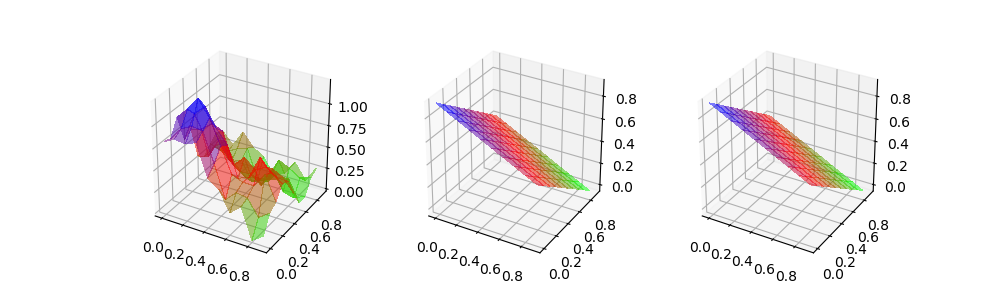
\includegraphics[width=1\linewidth]{images/surf/fake_linear_p01_n10.png}
  %\caption{}
  %\label{fig:v_x}
\end{subfigure}
\begin{subfigure}{\textwidth}
  \centering
  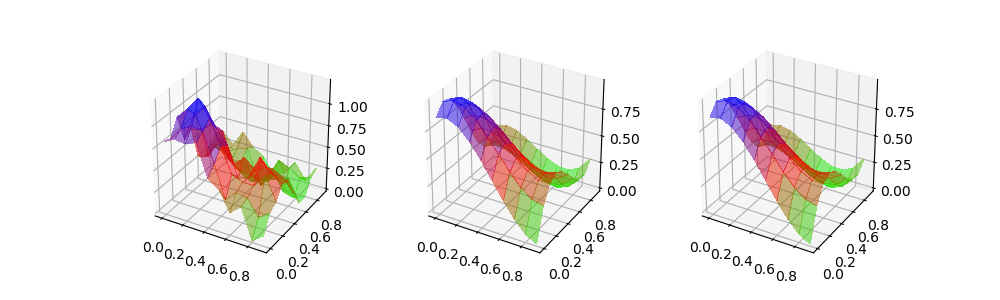
\includegraphics[width=1\linewidth]{images/surf/fake_linear_p03_n10.png}
  %\caption{}
  %\label{fig:vb_x}
\end{subfigure}
\begin{subfigure}{\textwidth}
  \centering
  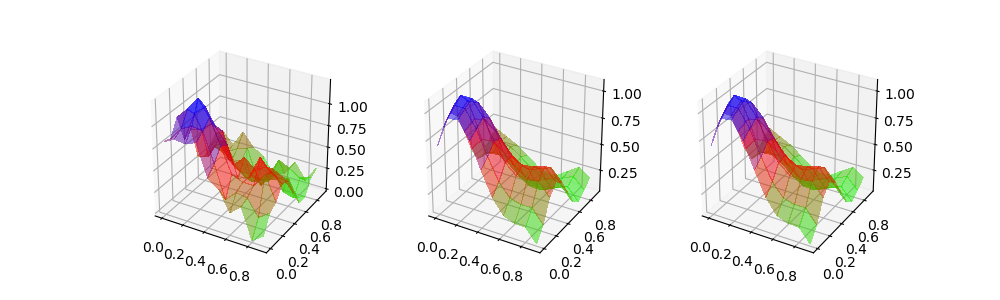
\includegraphics[width=1\linewidth]{images/surf/fake_linear_p05_n10.png}
  %\caption{}
  %\label{fig:v_x}
\end{subfigure}
\begin{subfigure}{\textwidth}
  \centering
  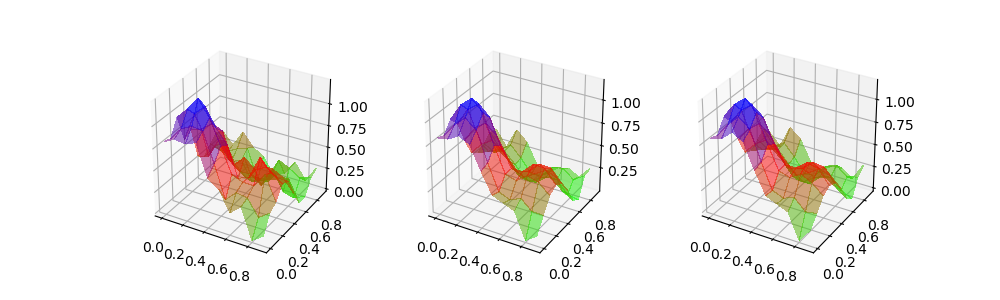
\includegraphics[width=1\linewidth]{images/surf/fake_linear_p08_n10.png}
  %\caption{}
  %\label{fig:v_x}
\end{subfigure}
\caption{The 3D visualisation of the noisy data set (left column) and the predicted surface via Lasso regression (right column) for polynomials 1, 3, 5 and 8 (from top to bottom). Grid is $10\times10$ points.}
\label{fig:linear-surf1}
\end{figure}

\begin{figure}[!ht]
\begin{subfigure}{\textwidth}
  \centering
  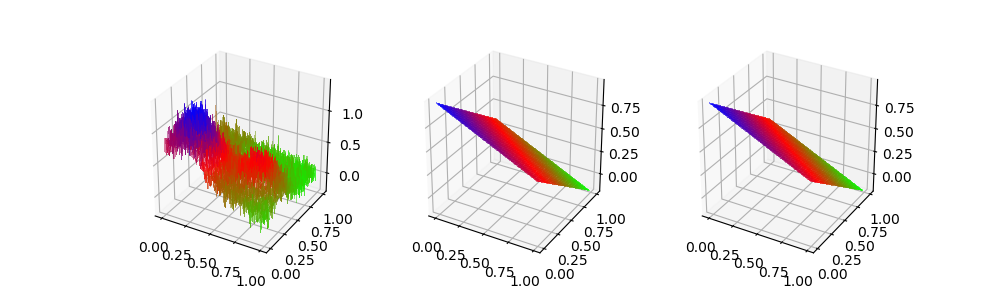
\includegraphics[width=1\linewidth]{images/surf/fake_linear_p01_n100.png}
  %\caption{}
  %\label{fig:v_x}
\end{subfigure}
\begin{subfigure}{\textwidth}
  \centering
  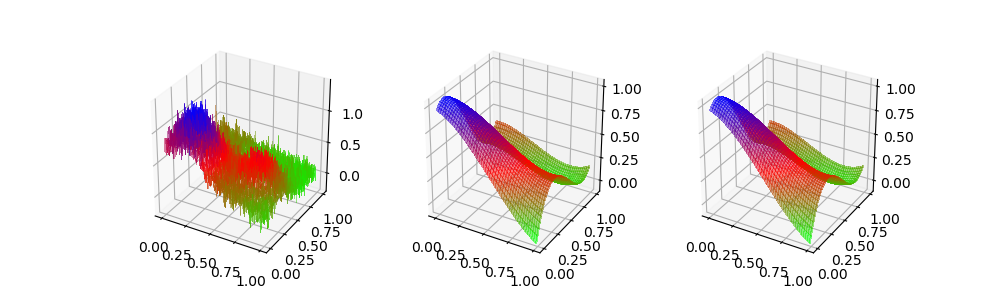
\includegraphics[width=1\linewidth]{images/surf/fake_linear_p03_n100.png}
  %\caption{}
  %\label{fig:vb_x}
\end{subfigure}
\begin{subfigure}{\textwidth}
  \centering
  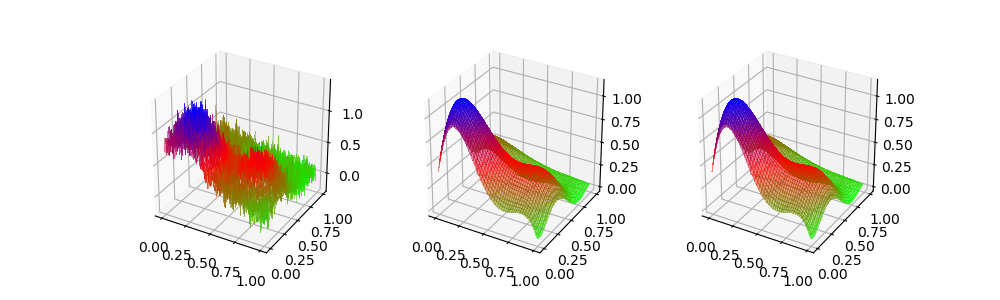
\includegraphics[width=1\linewidth]{images/surf/fake_linear_p05_n100.png}
  %\caption{}
  %\label{fig:v_x}
\end{subfigure}
\begin{subfigure}{\textwidth}
  \centering
  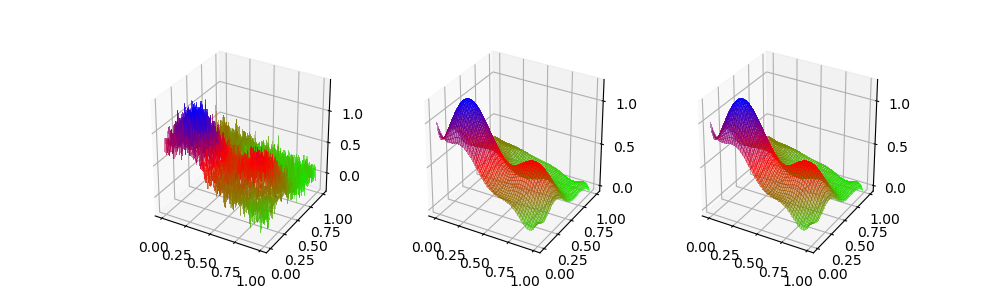
\includegraphics[width=1\linewidth]{images/surf/fake_linear_p08_n100.png}
  %\caption{}
  %\label{fig:v_x}
\end{subfigure}
\caption{The 3D visualisation of the noisy data set (left column) and the predicted surface via Lasso regression (right column) for polynomials 1, 3, 5 and 8 (from top to bottom). Grid is $100\times100$ points.}
\label{fig:linear-surf2}
\end{figure}
 
  \begin{figure}[!ht]
\begin{subfigure}{\textwidth}
  \centering
  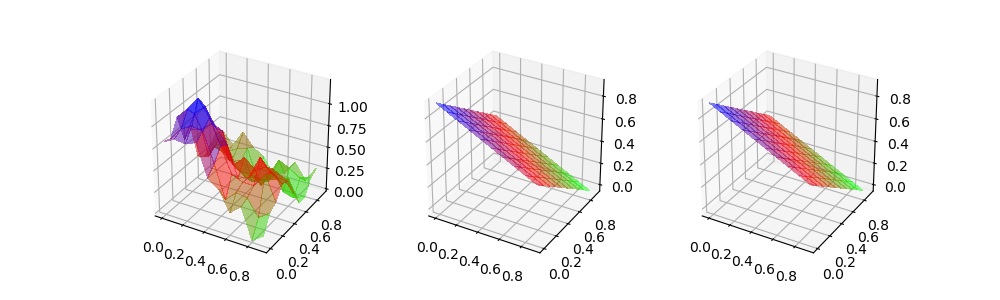
\includegraphics[width=1\linewidth]{images/surf/fake_ridge_p01_n10.png}
  %\caption{}
  %\label{fig:v_x}
\end{subfigure}
\begin{subfigure}{\textwidth}
  \centering
  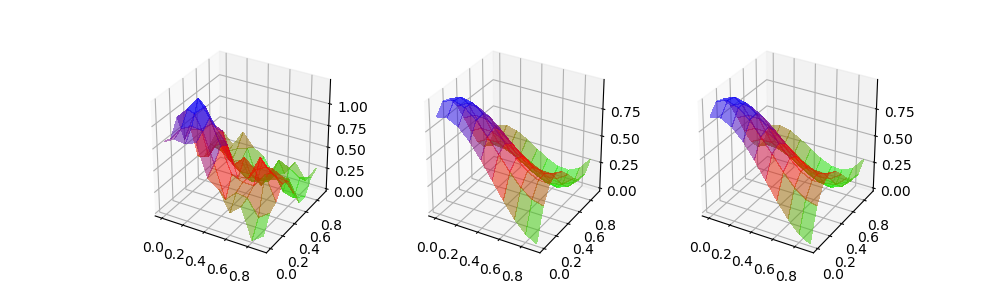
\includegraphics[width=1\linewidth]{images/surf/fake_ridge_p03_n10.png}
  %\caption{}
  %\label{fig:vb_x}
\end{subfigure}
\begin{subfigure}{\textwidth}
  \centering
  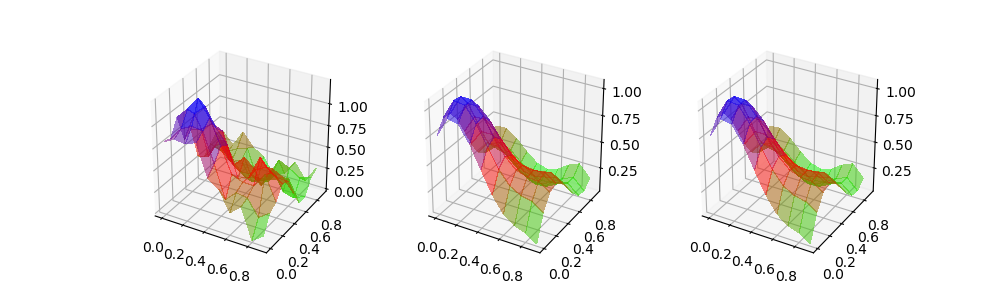
\includegraphics[width=1\linewidth]{images/surf/fake_ridge_p05_n10.png}
  %\caption{}
  %\label{fig:v_x}
\end{subfigure}
\begin{subfigure}{\textwidth}
  \centering
  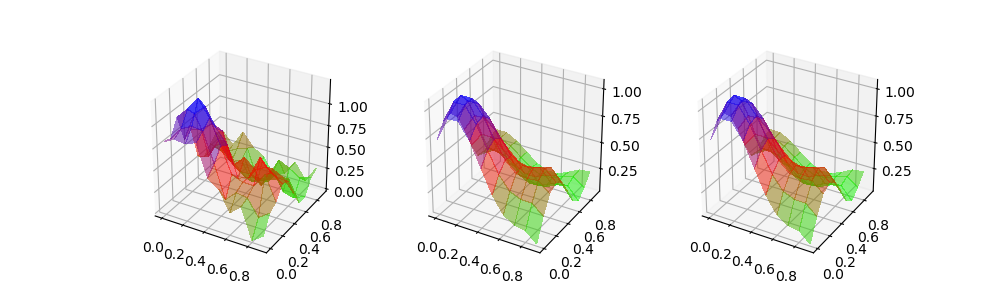
\includegraphics[width=1\linewidth]{images/surf/fake_ridge_p08_n10.png}
  %\caption{}
  %\label{fig:v_x}
\end{subfigure}
\caption{The 3D visualisation of the noisy data set (left column) and the predicted surface via Ridge regression (right column) for polynomials 1, 3, 5 and 8 (from top to bottom). Grid is $10\times10$ points and $\lambda = 0.0001$.}
\label{fig:ridge-surf1}
\end{figure}

 \begin{figure}[!ht]
\begin{subfigure}{\textwidth}
  \centering
  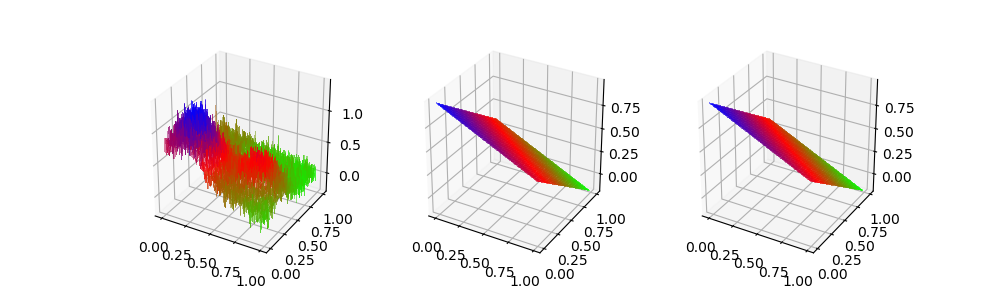
\includegraphics[width=1\linewidth]{images/surf/fake_ridge_p01_n100.png}
  %\caption{}
  %\label{fig:v_x}
\end{subfigure}
\begin{subfigure}{\textwidth}
  \centering
  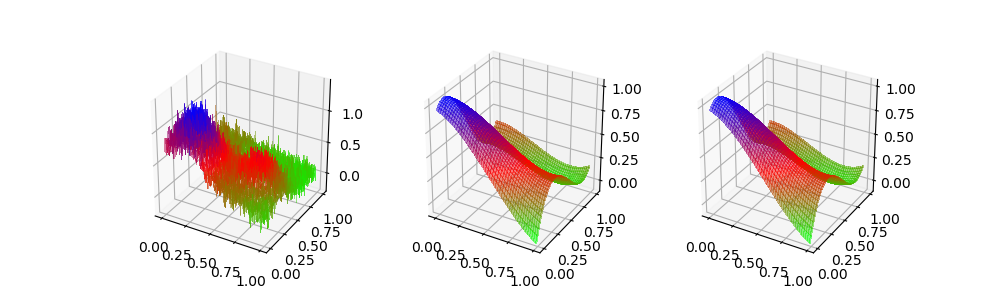
\includegraphics[width=1\linewidth]{images/surf/fake_ridge_p03_n100.png}
  %\caption{}
  %\label{fig:vb_x}
\end{subfigure}
\begin{subfigure}{\textwidth}
  \centering
  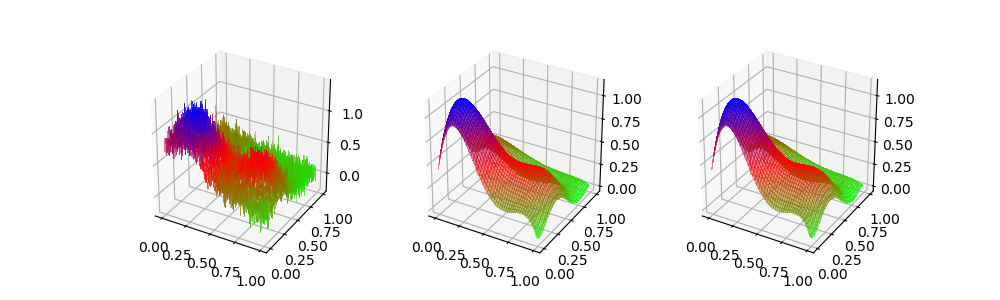
\includegraphics[width=1\linewidth]{images/surf/fake_ridge_p05_n100.png}
  %\caption{}
  %\label{fig:v_x}
\end{subfigure}
\begin{subfigure}{\textwidth}
  \centering
  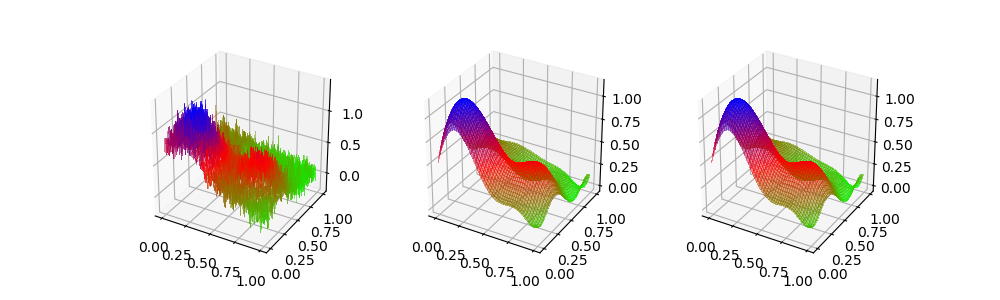
\includegraphics[width=1\linewidth]{images/surf/fake_ridge_p08_n100.png}
  %\caption{}
  %\label{fig:v_x}
\end{subfigure}
\caption{The 3D visualisation of the noisy data set (left column) and the predicted surface via Ridge regression (right column) for polynomials 1, 3, 5 and 8 (from top to bottom). Grid is $100\times100$ points and $\lambda = 0.0001$.}
\label{fig:ridge-surf2}
\end{figure}
 
\begin{figure}[!ht]
\begin{subfigure}{\textwidth}
  \centering
  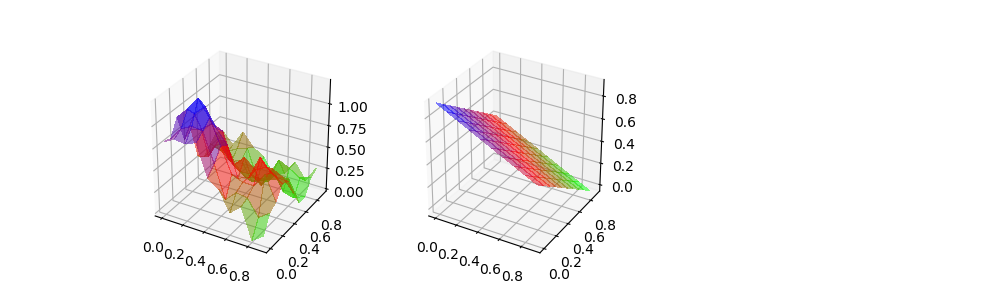
\includegraphics[width=1\linewidth]{images/surf/fake_lasso_p01_n10.png}
  %\caption{}
  %\label{fig:v_x}
\end{subfigure}
\begin{subfigure}{\textwidth}
  \centering
  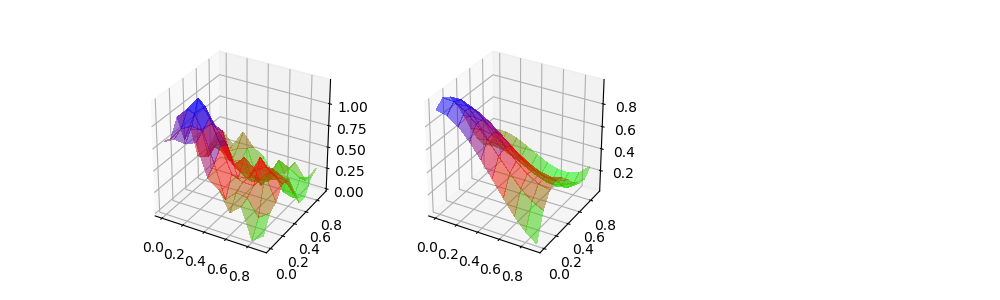
\includegraphics[width=1\linewidth]{images/surf/fake_lasso_p03_n10.png}
  %\caption{}
  %\label{fig:vb_x}
\end{subfigure}
\begin{subfigure}{\textwidth}
  \centering
  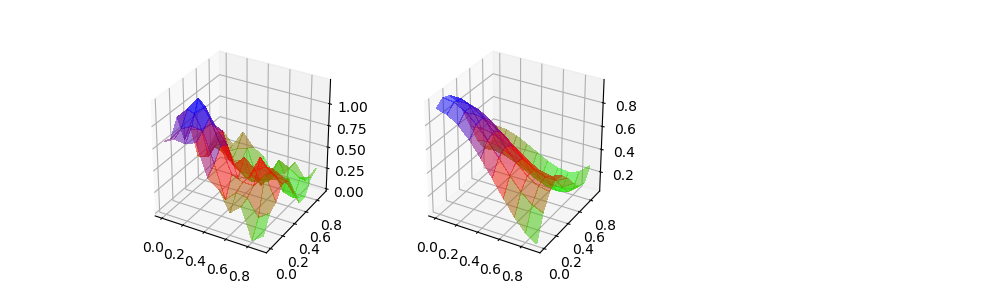
\includegraphics[width=1\linewidth]{images/surf/fake_lasso_p05_n10.png}
  %\caption{}
  %\label{fig:v_x}
\end{subfigure}
\begin{subfigure}{\textwidth}
  \centering
  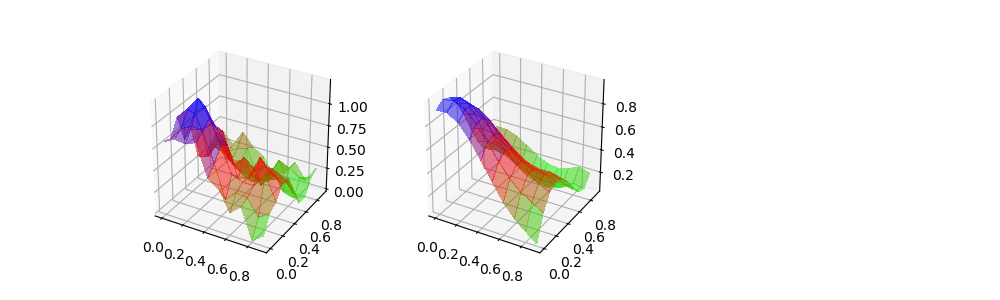
\includegraphics[width=1\linewidth]{images/surf/fake_lasso_p08_n10.png}
  %\caption{}
  %\label{fig:v_x}
\end{subfigure}
\caption{The 3D visualisation of the noisy data set (left column) and the predicted surface via Lasso regression (right column) for polynomials 1, 3, 5 and 8 (from top to bottom). Grid is $10\times10$ points and $\lambda = 0.0001$.}
\label{fig:lasso-surf1}
\end{figure}

\begin{figure}[!ht]
\begin{subfigure}{\textwidth}
  \centering
  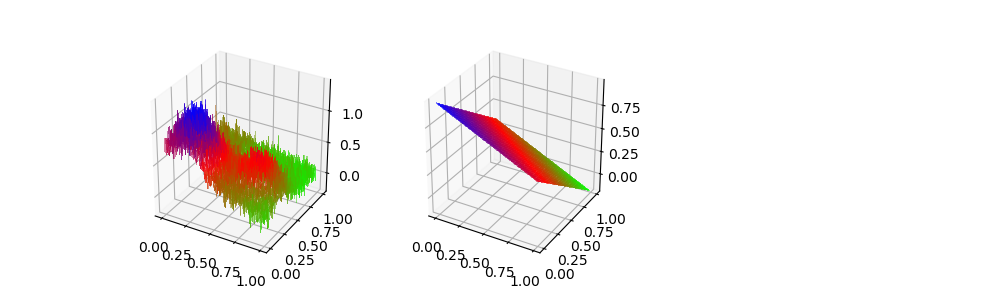
\includegraphics[width=1\linewidth]{images/surf/fake_lasso_p01_n100.png}
  %\caption{}
  %\label{fig:v_x}
\end{subfigure}
\begin{subfigure}{\textwidth}
  \centering
  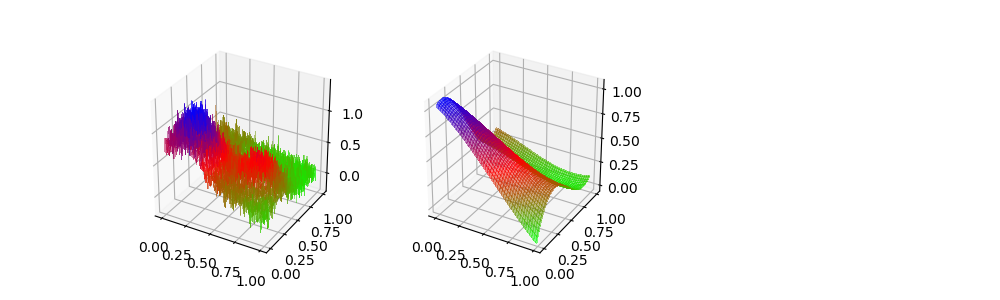
\includegraphics[width=1\linewidth]{images/surf/fake_lasso_p03_n100.png}
  %\caption{}
  %\label{fig:vb_x}
\end{subfigure}
\begin{subfigure}{\textwidth}
  \centering
  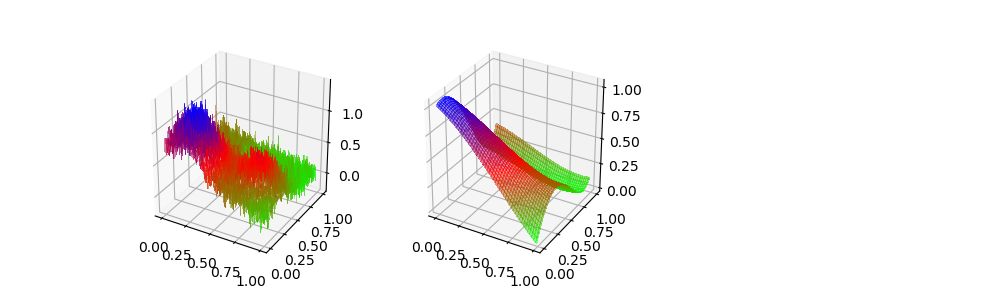
\includegraphics[width=1\linewidth]{images/surf/fake_lasso_p05_n100.png}
  %\caption{}
  %\label{fig:v_x}
\end{subfigure}
\begin{subfigure}{\textwidth}
  \centering
  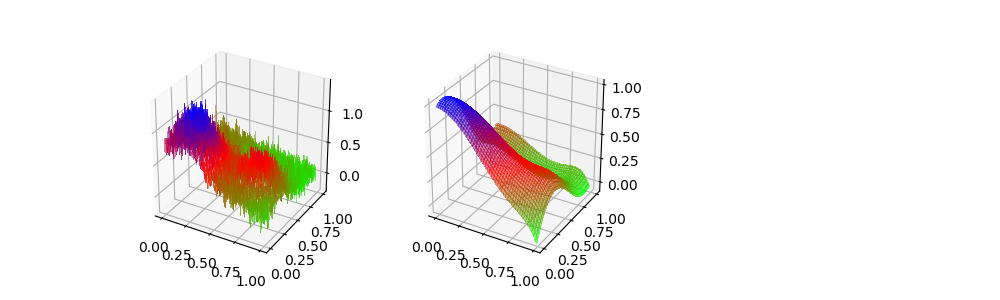
\includegraphics[width=1\linewidth]{images/surf/fake_lasso_p08_n100.png}
  %\caption{}
  %\label{fig:v_x}
\end{subfigure}
\caption{The 3D visualisation of the noisy data set (left column) and the predicted surface via Lasso regression (right column) for polynomials 1, 3, 5 and 8 (from top to bottom). Grid is $100\times100$ points and $\lambda = 0.0001$.}
\label{fig:lasso-surf2}
\end{figure}

%%%%%%%%%%%%%%%%%%%%%%%%%%%%%%%%%%%%%%%%%%%%%%%%%%%%%%%%%%%%%%%%%%%%%%%%%%%%%%%%%%%%%
% betas
%%%%%%%%%%%%%%%%%%%%%%%%%%%%%%%%%%%%%%%%%%%%%%%%%%%%%%%%%%%%%%%%%%%%%%%%%%%%%%%%%%%%%

\begin{figure}[!ht]
\begin{subfigure}{\textwidth}
  \centering
  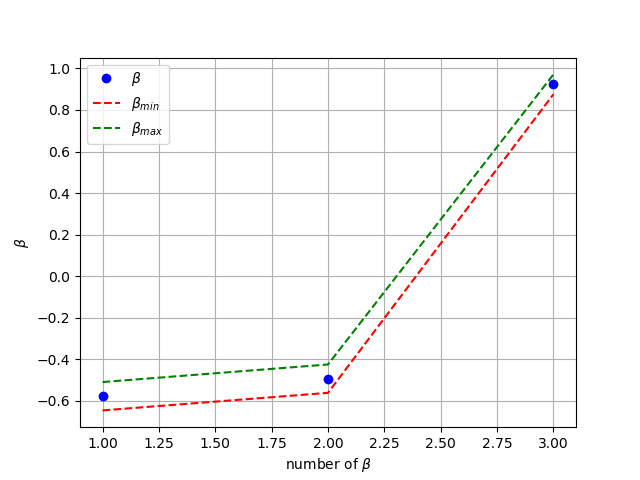
\includegraphics[width=0.5\linewidth]{images/betas/fake_linear_beta_p01_n10.png}
  %\caption{}
  %\label{fig:v_x}
\end{subfigure}
\begin{subfigure}{\textwidth}
  \centering
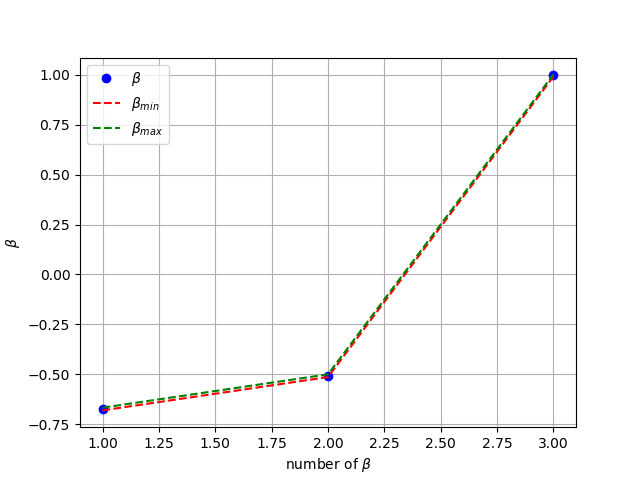
\includegraphics[width=0.5\linewidth]{images/betas/fake_linear_beta_p01_n100.png}
  %\caption{}
  %\label{fig:vb_x}
\end{subfigure}
\begin{subfigure}{\textwidth}
  \centering
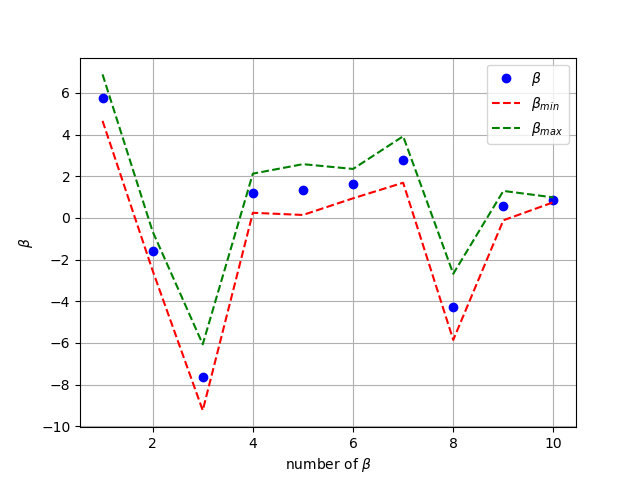
\includegraphics[width=0.5\linewidth]{images/betas/fake_linear_beta_p03_n10.png}
  %\caption{}
  %\label{fig:v_x}
\end{subfigure}
\begin{subfigure}{\textwidth}
  \centering
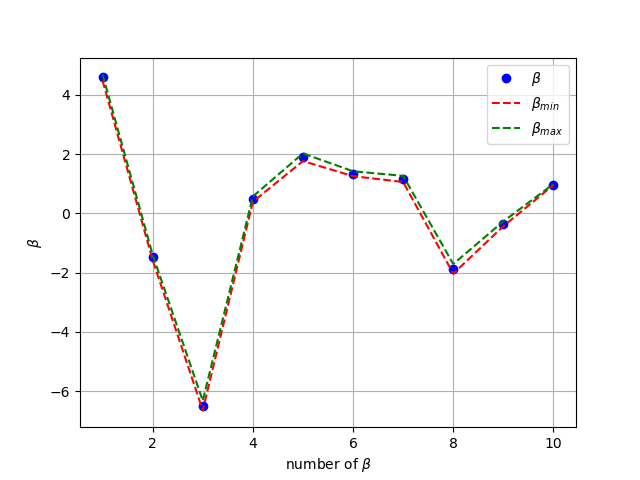
\includegraphics[width=0.5\linewidth]{images/betas/fake_linear_beta_p03_n100.png}
  %\caption{}
  %\label{fig:v_x}
\end{subfigure}
\begin{subfigure}{\textwidth}
  \centering
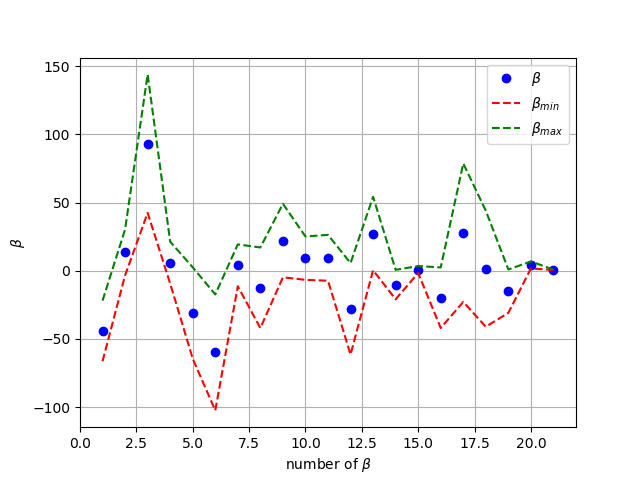
\includegraphics[width=0.5\linewidth]{images/betas/fake_linear_beta_p05_n10.png}
  %\caption{}
  %\label{fig:v_x}
\end{subfigure}
\begin{subfigure}{\textwidth}
  \centering
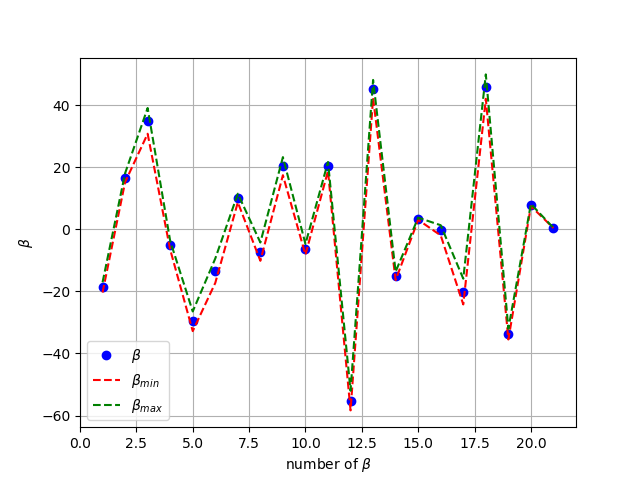
\includegraphics[width=0.5\linewidth]{images/betas/fake_linear_beta_p05_n100.png}
  %\caption{}
  %\label{fig:v_x}
\end{subfigure}
\begin{subfigure}{\textwidth}
  \centering
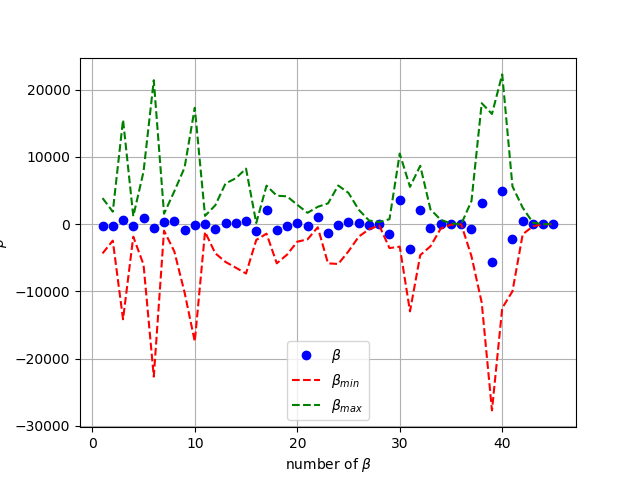
\includegraphics[width=0.5\linewidth]{images/betas/fake_linear_beta_p08_n10.png}
  %\caption{}
  %\label{fig:v_x}
\end{subfigure}
\begin{subfigure}{\textwidth}
  \centering
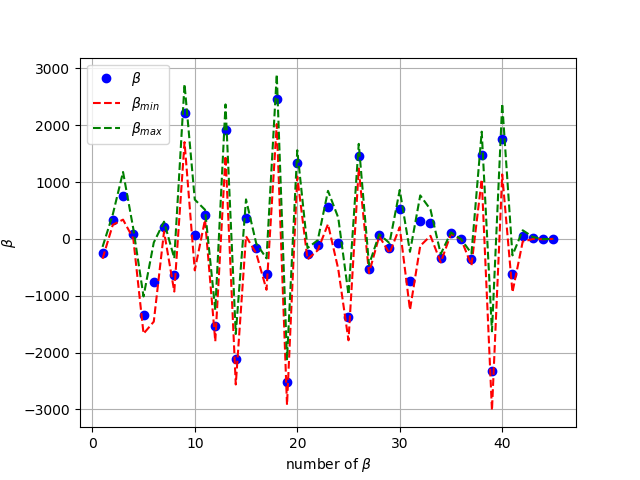
\includegraphics[width=0.5\linewidth]{images/betas/fake_linear_beta_p08_n100.png}
  %\caption{}
  %\label{fig:v_x}
\end{subfigure}
\caption{Manually calculated parameters $\beta$ of Linear Regression model for polynomials 1, 3, 5 and 8 (from top to bottom) on the grids $10\times10$ (left column) and $100\times100$ (right column) points.}
\label{fig:linear-beta}
\end{figure}

\begin{figure}[!ht]
\begin{subfigure}{\textwidth}
  \centering
  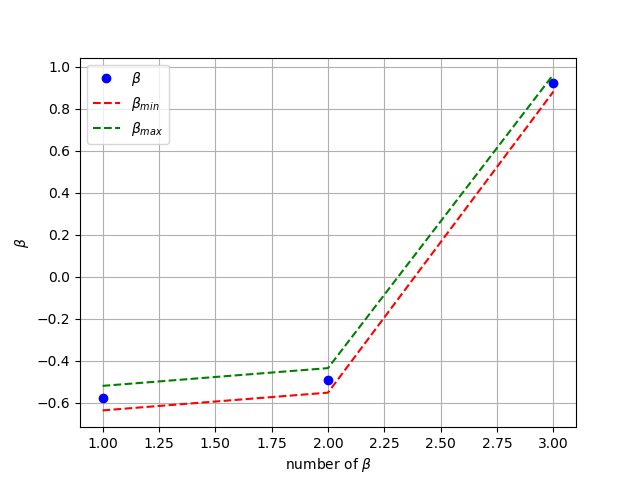
\includegraphics[width=0.5\linewidth]{images/betas/fake_ridge_beta_p01_n10.png}
  %\caption{}
  %\label{fig:v_x}
\end{subfigure}
\begin{subfigure}{\textwidth}
  \centering
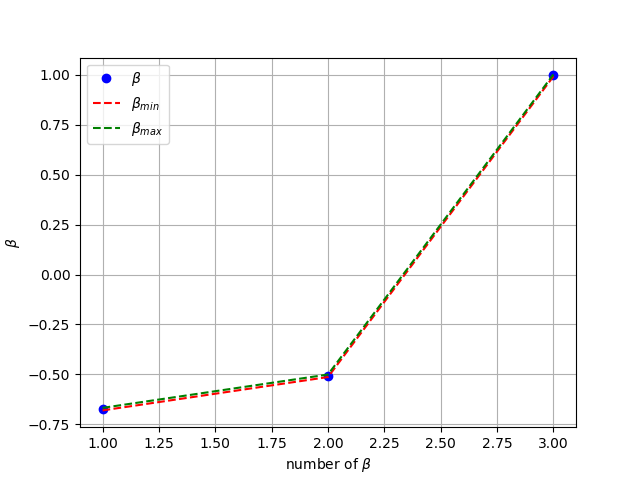
\includegraphics[width=0.5\linewidth]{images/betas/fake_ridge_beta_p01_n100.png}
  %\caption{}
  %\label{fig:vb_x}
\end{subfigure}
\begin{subfigure}{\textwidth}
  \centering
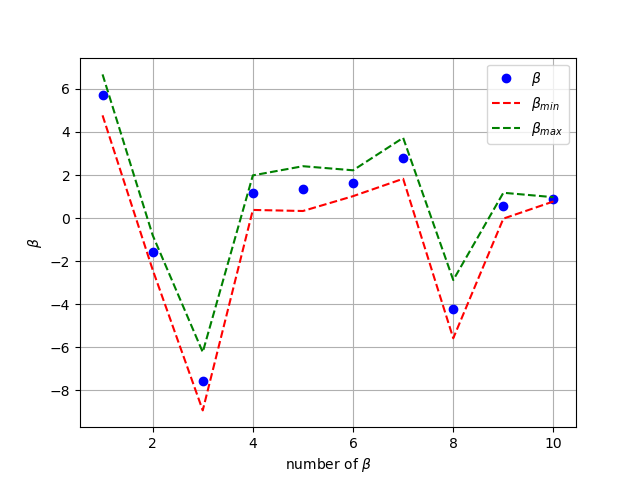
\includegraphics[width=0.5\linewidth]{images/betas/fake_ridge_beta_p03_n10.png}
  %\caption{}
  %\label{fig:v_x}
\end{subfigure}
\begin{subfigure}{\textwidth}
  \centering
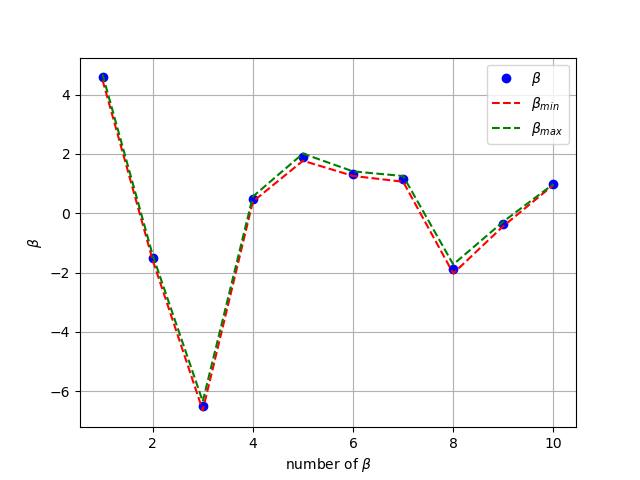
\includegraphics[width=0.5\linewidth]{images/betas/fake_ridge_beta_p03_n100.png}
  %\caption{}
  %\label{fig:v_x}
\end{subfigure}
\begin{subfigure}{\textwidth}
  \centering
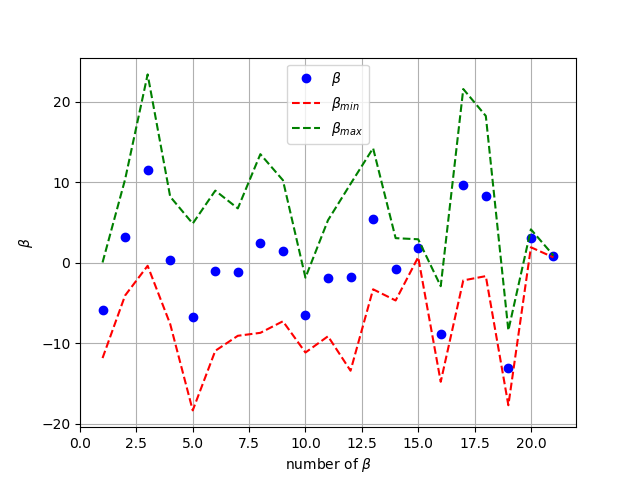
\includegraphics[width=0.5\linewidth]{images/betas/fake_ridge_beta_p05_n10.png}
  %\caption{}
  %\label{fig:v_x}
\end{subfigure}
\begin{subfigure}{\textwidth}
  \centering
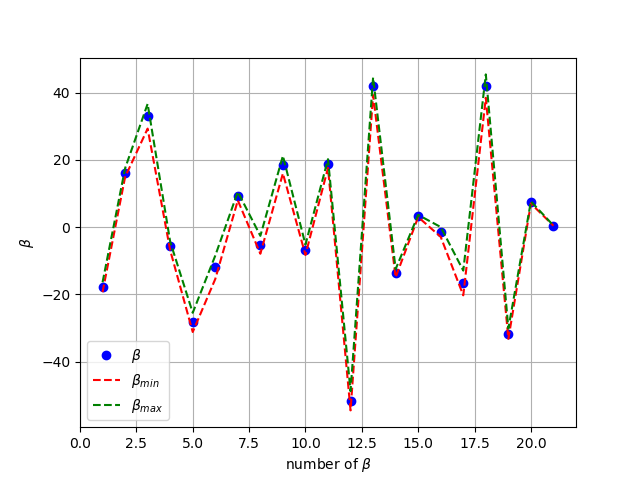
\includegraphics[width=0.5\linewidth]{images/betas/fake_ridge_beta_p05_n100.png}
  %\caption{}
  %\label{fig:v_x}
\end{subfigure}
\begin{subfigure}{\textwidth}
  \centering
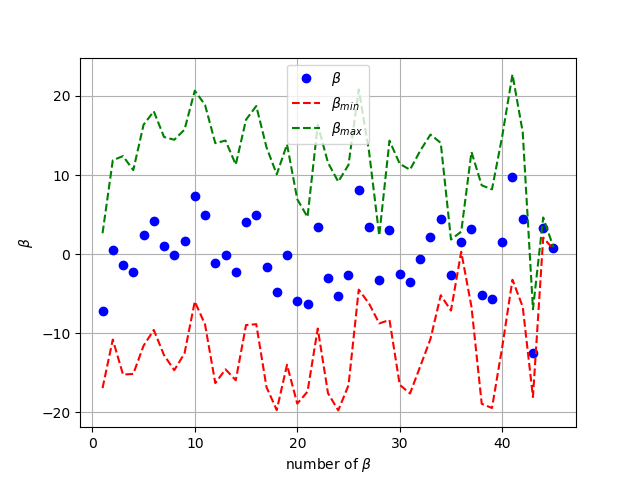
\includegraphics[width=0.5\linewidth]{images/betas/fake_ridge_beta_p08_n10.png}
  %\caption{}
  %\label{fig:v_x}
\end{subfigure}
\begin{subfigure}{\textwidth}
  \centering
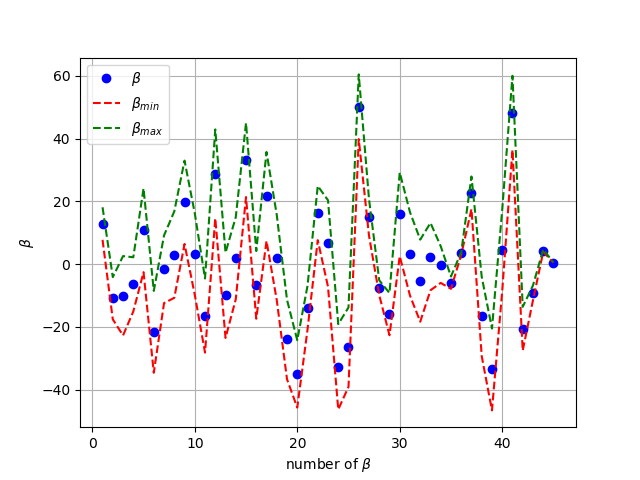
\includegraphics[width=0.5\linewidth]{images/betas/fake_ridge_beta_p08_n100.png}
  %\caption{}
  %\label{fig:v_x}
\end{subfigure}
\caption{Manually calculated parameters $\beta$ of Ridge Regression model for polynomials 1, 3, 5 and 8 (from top to bottom) on the grids $10\times10$ (left column) and $100\times100$ (right column) points. $\lambda = 0.0001$.}
\label{fig:ridge-beta}
\end{figure}

Figures \ref{fig:linear-beta} and \ref{fig:ridge-beta} clearly state that the more points we have in the data set, the less uncertain we be about out model parameters.


Unfortunately, all these values cannot say for sure whether we will fit future data sets correctly (our main goal is to create such model) or not. That is why, as was discussed in the previous sections, we need to consider a resampling techniques. 

 \subsubsection{Resampling techniques: Bias-variance tradeoff}
 
 In section \ref{} I have described implementation of kFold Cross Validation Algorithm; thus, below I present the main results for the specified runs.
 
 Figure \rf{} shows that when the amount of points increases the closer test slope appears to be to the white noise threshold (in our case supposed to be at $\sigma^2=0.01$), and less diverge it from the train values. On the contrary, the less amount of points we have the more evident is the \textit{bias-variance trade-off}: the area to the left is the \textit{High Bias} (\textit{Low Variance}) zone, whereas with the increase of model complexity the curves are diverging, while entering \textit{Low Bias} (\textit{High Variance}) zone.
 
 %%%%%%%%%%%%%%%%%%%%%%%%%%%%%%%%%%%%%%%%%%%%%%%%%%%%%%%%%%%%%%%%%%%%%%%%%%%%%%%%%%%%%
 % MSE
 %%%%%%%%%%%%%%%%%%%%%%%%%%%%%%%%%%%%%%%%%%%%%%%%%%%%%%%%%%%%%%%%%%%%%%%%%%%%%%%%%%%%%
\begin{figure}[!ht]
\begin{subfigure}{\textwidth}
  \centering
  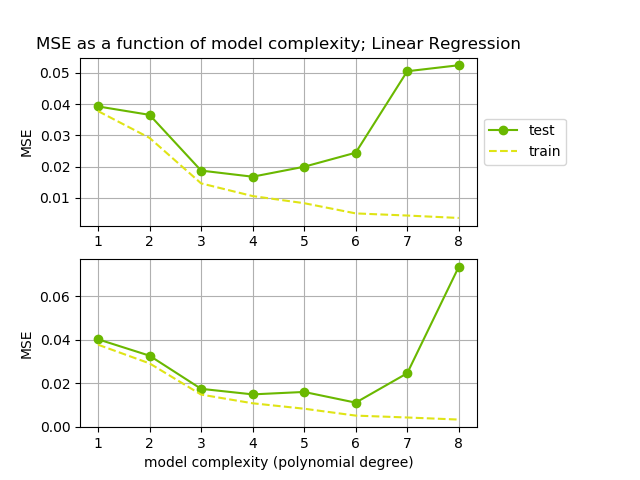
\includegraphics[width=0.55\linewidth]{images/mse/fake_linear_mse_p08_n10.png}
  %\caption{$10\times10$}
  %\label{fig:v_x}
\end{subfigure}
\begin{subfigure}{\textwidth}
  \centering
  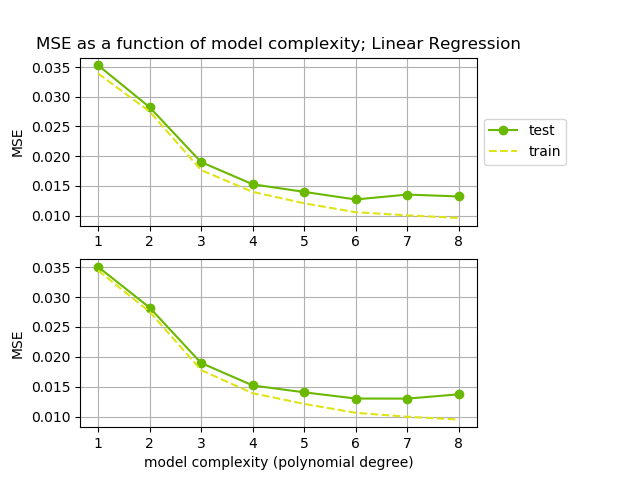
\includegraphics[width=0.55\linewidth]{images/mse/fake_linear_mse_p08_n21.png}
  %\caption{$21\times21$}
  %\label{fig:vb_x}
\end{subfigure}
\begin{subfigure}{\textwidth}
  \centering
  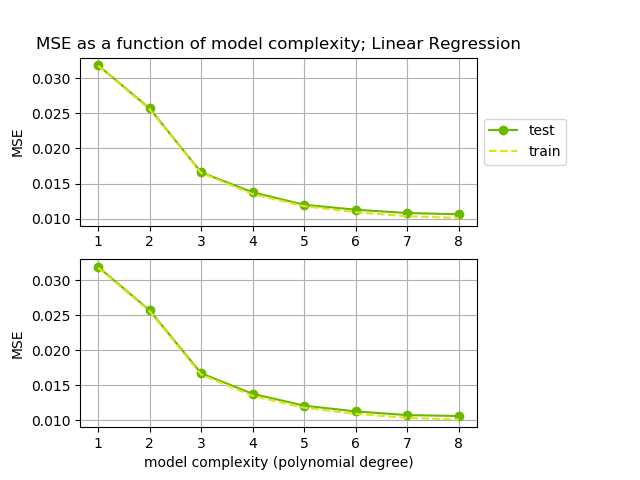
\includegraphics[width=0.55\linewidth]{images/mse/fake_linear_mse_p08_n50.png}
  %\caption{$50\times50$}
  %\label{fig:vb_x}
\end{subfigure}
\begin{subfigure}{\textwidth}
  \centering
  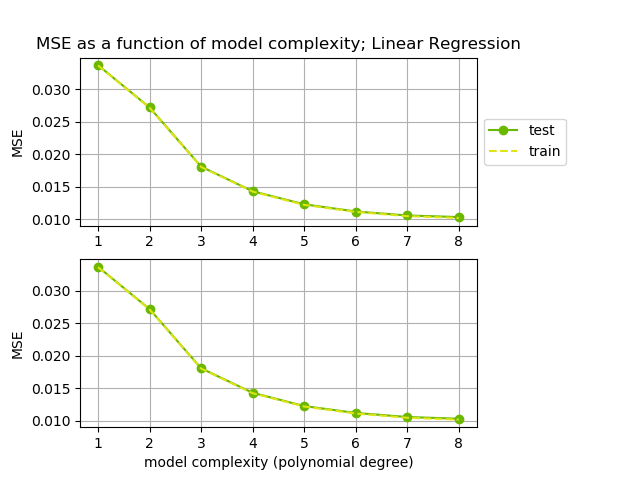
\includegraphics[width=0.55\linewidth]{images/mse/fake_linear_mse_p08_n100.png}
  %\caption{$100\times100$}
  %\label{fig:vb_x}
\end{subfigure}
\caption{MSE plot of train and test data sets as a function of model complexity (polynomial degree) calculated via Linear Regression for several different grids: $10\times10$ (top left), $21\times21$ (top right), $50\times50$ (bottom left), $100\times100$ (bottom right).}
\label{fig:linear-mse}
\end{figure}

\begin{figure}[!ht]
\begin{subfigure}{\textwidth}
  \centering
  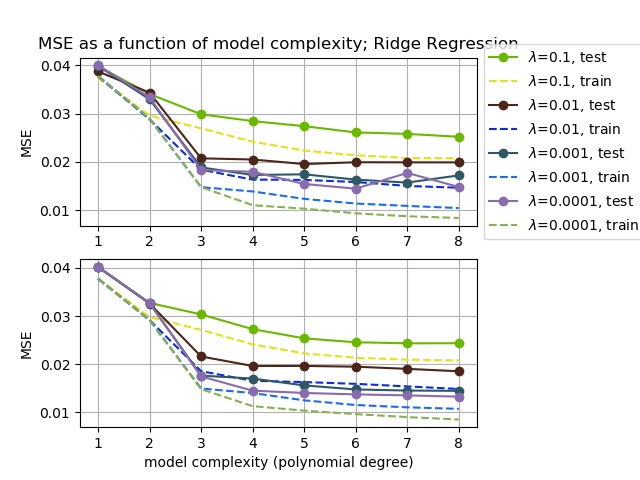
\includegraphics[width=0.55\linewidth]{images/mse/fake_ridge_mse_p08_n10.png}
  %\caption{$10\times10$}
  %\label{fig:v_x}
\end{subfigure}
\begin{subfigure}{\textwidth}
  \centering
  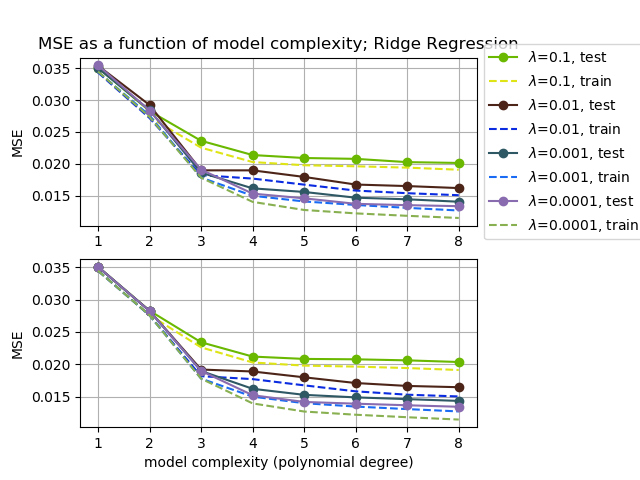
\includegraphics[width=0.55\linewidth]{images/mse/fake_ridge_mse_p08_n21.png}
  %\caption{$21\times21$}
  %\label{fig:vb_x}
\end{subfigure}
\begin{subfigure}{\textwidth}
  \centering
  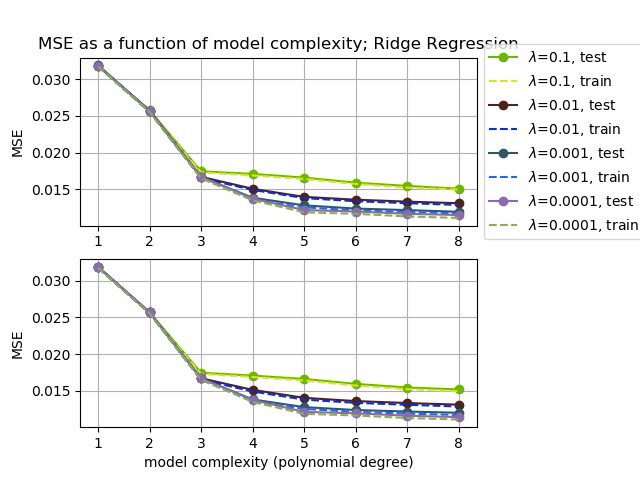
\includegraphics[width=0.55\linewidth]{images/mse/fake_ridge_mse_p08_n50.png}
  %\caption{$50\times50$}
  %\label{fig:vb_x}
\end{subfigure}
\begin{subfigure}{\textwidth}
  \centering
  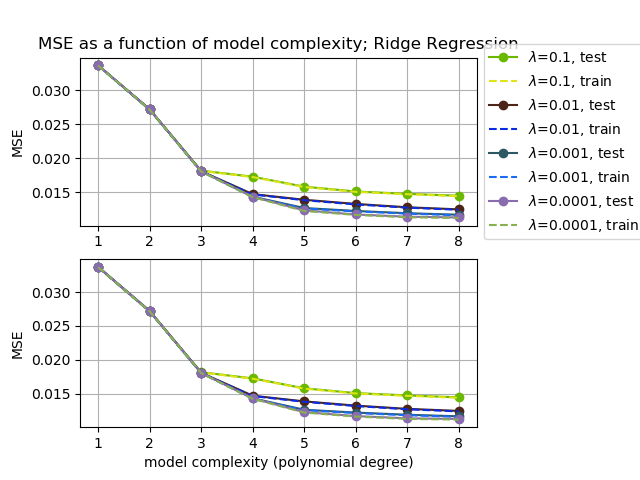
\includegraphics[width=0.55\linewidth]{images/mse/fake_ridge_mse_p08_n100.png}
  %\caption{$100\times100$}
  %\label{fig:vb_x}
\end{subfigure}
\caption{MSE plot of train and test data sets as a function of model complexity (polynomial degree) calculated via Ridge Regression for several different grids: $10\times10$ (top left), $21\times21$ (top right), $50\times50$ (bottom left), $100\times100$ (bottom right). $\lambda_i = 0.1$, $0.01$ and $0.0001$.}
\label{fig:ridge-mse}
\end{figure}

\begin{figure}[!ht]
\begin{subfigure}{\textwidth}
  \centering
  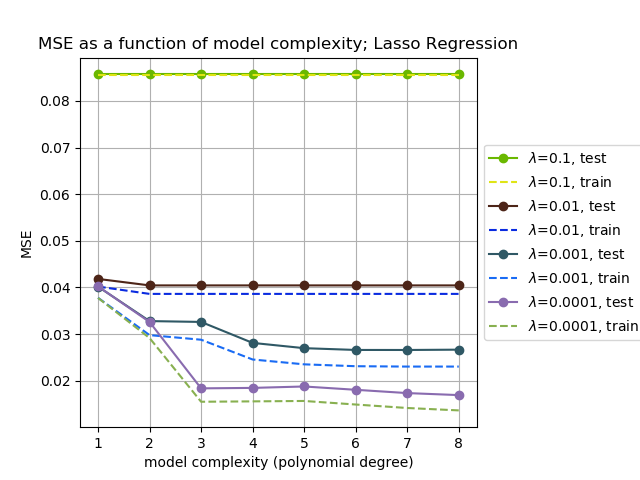
\includegraphics[width=0.55\linewidth]{images/mse/fake_lasso_mse_p08_n10.png}
  %\caption{$10\times10$}
  %\label{fig:v_x}
\end{subfigure}
\begin{subfigure}{\textwidth}
  \centering
  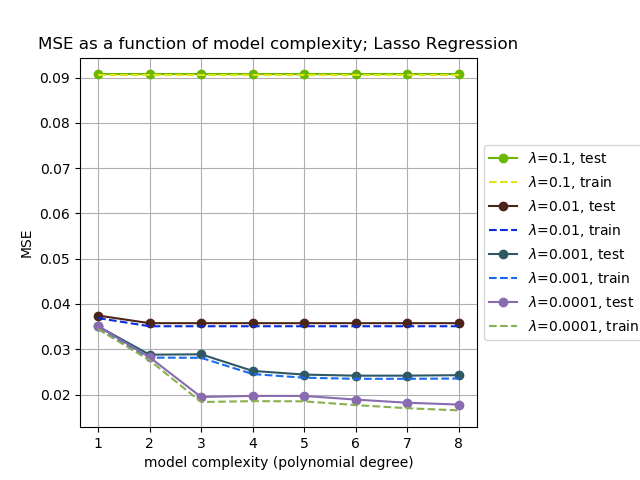
\includegraphics[width=0.55\linewidth]{images/mse/fake_lasso_mse_p08_n21.png}
  %\caption{$21\times21$}
  %\label{fig:vb_x}
\end{subfigure}
\begin{subfigure}{\textwidth}
  \centering
  \includegraphics[width=0.55\linewidth]{images/mse/fake_lasso_mse_p08_n50.png}
  %\caption{$50\times50$}
  %\label{fig:vb_x}
\end{subfigure}
\begin{subfigure}{\textwidth}
  \centering
  \includegraphics[width=0.55\linewidth]{images/mse/fake_lasso_mse_p08_n100.png}
  %\caption{$100\times100$}
  %\label{fig:vb_x}
\end{subfigure}
\caption{MSE plot of train and test data sets as a function of model complexity (polynomial degree) calculated via Lasso Regression for several different grids: $10\times10$ (top left), $21\times21$ (top right), $50\times50$ (bottom left), $100\times100$ (bottom right). $\lambda_i = 0.1$, $0.01$ and $0.0001$.}
\label{fig:lasso-mse}
\end{figure}

As we can see from figure \rf{}, the closer hyper parameter to zero, the closer the values of Ridge regression correlate with the values from Linear regression. And vice versa, the closer $\lambda$ to 1, the more straight our line appear to be - this is nothing surprising, as setting $\lambda=1$ equivalent to setting $\beta\rightarrow\infty$ (?) <= to zero (check lasso once again, it should be zero).

The figure \rf{} shows MSE for training and test data sets, calculated via Lasso regression and kFold cross validation, when I split data sets into 5 folds. It is evident that Lasso appears to be more dependent on hyper parameter, then Ridge regression.

From a student view about Lasso:
\textit{"The problem is that there is no problem. This is just truly what the data is like: the dataset is so large that the signal to noise ratio is very high, this means that even with high polynomial orders you never overfit (because you have so much training and test data that they become very similar).}

\texdtit{When we use a lot smaller amount of data points, for example 500, then we see the expected result where the test error goes up after a number of rounds.}

\textit{It makes sense that when you turn off shuffle the training and test error increases: without shuffle, the training data is one part of the image, and the test data a different part of the image. Obviously you can not "learn" something that you have not seen."}




 \subsection{Real Data}
 
 Below I present main results for the real data set. I run script up til 5th polynomial degree with several different hyper parameters.
 
 \begin{figure}[!ht]
\begin{subfigure}{\textwidth}
  \centering
  \includegraphics[width=1.2\linewidth]{images/surf/fake_lasso_p01_n50.png}
  %\caption{}
  %\label{fig:v_x}
\end{subfigure}
\begin{subfigure}{\textwidth}
  \centering
  \includegraphics[width=1.2\linewidth]{images/surf/fake_lasso_p03_n50.png}
  %\caption{}
  %\label{fig:vb_x}
\end{subfigure}
\begin{subfigure}{\textwidth}
  \centering
  \includegraphics[width=1.2\linewidth]{images/surf/fake_lasso_p05_n50.png}
  %\caption{}
  %\label{fig:v_x}
\end{subfigure}
\caption{The 3D visualisation of the noisy data set (left column) and the predicted surface via Lasso regression (right column) for polynomials 1, 3, 5 and 8 (from top to bottom). Grid is $50\times50$ points and $\lambda = 0.0001$.}
\label{fig:lasso-surf}
\end{figure}
 
 \subsection{Future Improvements}
 
 This question is more of general nature, where I mostly summarize the things which would be good to implement, but due to lack of time was not implemented:
 
 - Tuning of the Ridge and lasso, e.g. GridSearchCV
 - Reduce the size of the data set, without losing the information. Huffman coding as a solution?
 - Add features which will support any type of input function (say with n independent variables - it can be an input one) <= would be fun.
 - The Multiprocessing was implemented, but it is not perfect <= think of a better way to do it;
 
 As one of the future improvements, It woulde be better to implement the tuning of the Ridge and Lasso models. To be more precise, generate, say, hundred $\lambda$ values and find the corresponding MSEs for each of them. after that, find the minimal one out of 100 generated - this value will be give us the best $\lambda$ value for Ridge and Lasso Regressions. I wanted to implement this feature already, but due to the high value of real data sets, it will take a lot of time to converge even for one polynomial. 
 
 One of the students suggest reduce the size of the data set without losing information. Perhaps, it is good approach in general, say use Huffman coding or something similar ?



\section{Conclusions}
\label{sec:conclusions}

%\textit{Conclusions, discussions and critical comments: on what was learned about the method used and on the results obtained. Possible directions and future improvements?}

During this project, I have written a self-consistent code, which implements several regression algorithms on both pre-generated data and real data. Moreover, it also computes kFold cross validation (with k=5) with manual code on both Linear and ridge Regressions and also computes the code with the use of Scikit learn standard methods for every regression method discussed in this report.

As outputs, program creates a bunch of "png" and "txt" files which are stored inside Output folder (in the directory where script is located). 

Because I haven't accounted for the amount of points present in the real data set, I wasted a lot of time waiting for the script to finish its work. Therefore, I enabled the possibility to use only part of the data set (e.g. $10\%$). However, based on what I saw so far, for the system with very \textit{large amount of points}, \textit{OLS} would be more than enough to fit the model, whereas for \textit{lesser amount of points} (when bias-variance trade of is quite prominent), the better model is \textit{Ridge} Regression. the problem with Lasso regression is that you need to be quite careful to tun your model with correct $\lambda$ first.

Although the program runs without crashing, there are several possible improvements, which would be good to implement in observable future:
\begin{itemize}
    \item Reduce the size of the data set without losing  information. During one of the discussions on Piazza, one of the students mentioned possibility to reduce the size of the data set. He/she even mentioned the code snippet which can be used for this and, although I am not sure whether his/her solution is good, the idea itself is very good. If this code doesn't work, maybe I will try to implement something like Huffman Coding or similar thing;
    \item Better Parallelization. Although I have already implemented this feature, it only works now for calculation of kFold cross validation for various parameters of $\lambda$. I'd like it to be expanded on the entire script;
    \item One more possible solution I thought of to reduce the time, I can simply split the calculating of KFolds and Regression analysis into separate runs. For instance, right now I am running the entire pipeline, i.e. Polynomial, Ridge, Lasso regressions with its respective Scikit learn analogs. So the idea is to be able to run the code for only one or two methods at once, and if, the user really wants to, run the entire code with all methods implemented;
\end{itemize}
%%%%%%%%%%%%%%%%%%%%%%%%%%%%%%%%%%%%%%%%%%%%%%%%%%%%%%%%%

% References

% Appendix (additional figures and codes)

\end{document}
